\section{敏感方向的正则化与截断}
\label{sec:ls-truncated-svd-ridge}

上一节表明，数据误差沿小奇异值方向被放大$1/\sigma_i$倍。QR等正交算法只能避免在问题本身的敏感度之外再损失精度，改变不了这种放大。本节换一种做法：通过惩罚系数的大小或舍弃部分方向，主动修改求解目标，用一部分拟合误差换取解的稳定。下面先给出岭回归与Tikhonov正则化，再给出截断SVD，并分别说明计算路线与所作的取舍。

\subsection{岭回归与Tikhonov正则化}
\label{sec:ls-regularized-ls}

\paragraph{目标与可解条件}
对$\lambda>0$，\term{岭回归}（ridge regression）求解
\begin{equation}
 \min_{\bm x}\ \lVert\bm A\bm x-\bm b\rVert_2^2+\lambda\lVert\bm x\rVert_2^2 .
 \label{eq:ls-ridge-objective}
\end{equation}
惩罚也可以作用在希望压小的量$\bm L\bm x$上，$\bm L\in\mathbb R^{p\times d}$，例如相邻分量之差，目标改为$\lVert\bm A\bm x-\bm b\rVert_2^2+\lambda\lVert\bm L\bm x\rVert_2^2$，称为\term{Tikhonov正则化}（Tikhonov regularization）\scite{math-hansen2008regtools}，岭回归是$\bm L=\bm I$的情形。两项平方长度之和等于把两个残差向量上下堆叠后的平方长度，所以它是一个\term{增广最小二乘}（augmented least squares）问题
\begin{equation}
 \min_{\bm x}\lVert\bm F\bm x-\bm c\rVert_2^2,\qquad
 \bm F=\begin{bmatrix}\bm A\\ \sqrt\lambda\,\bm L\end{bmatrix},\quad
 \bm c=\begin{bmatrix}\bm b\\ \bm0\end{bmatrix}.
 \label{eq:ls-augmented-system}
\end{equation}
由此可以直接读出解的存在性与唯一性。

\begin{theorem}[Tikhonov解的存在与唯一]
\label{thm:ls-tikhonov-existence-uniqueness}
设$\bm A\in\mathbb R^{m\times d}$，$\bm L\in\mathbb R^{p\times d}$，$\lambda>0$。Tikhonov目标的极小点恰为方程
\[
 (\bm A^\top\bm A+\lambda\bm L^\top\bm L)\bm x=\bm A^\top\bm b
\]
的解，这样的解总存在；解唯一当且仅当
\begin{equation}
 \ker\bm A\cap\ker\bm L=\{\bm0\}.
 \label{eq:linear-algebra-tikhonov-common-nullspace}
\end{equation}
特别地，岭回归对任意$\bm A$都有唯一解。
\end{theorem}
\begin{proof}
目标等于增广问题~\eqref{eq:ls-augmented-system}，由第~\ref{sec:ls-ordinary-ls}节，它的极小点恰为正规方程$\bm F^\top\bm F\bm x=\bm F^\top\bm c$的解，总存在，且唯一当且仅当$\ker\bm F=\{\bm0\}$。代入$\bm F,\bm c$即得上面的方程。$\lambda>0$时$\bm F\bm x=\bm0$等价于$\bm A\bm x=\bm0$且$\bm L\bm x=\bm0$，所以$\ker\bm F=\ker\bm A\cap\ker\bm L$。岭回归中$\ker\bm I=\{\bm0\}$。
\end{proof}

一般的$\bm L$未必满足条件~\eqref{eq:linear-algebra-tikhonov-common-nullspace}：$\bm A=\bm L=[\,1\ \ -1\,]$时，$(1,1)^\top$方向既不影响拟合也不受惩罚，无论$\lambda$多大都定不下两个分量的共同水平。加入惩罚以后，目标中的平方不能去掉：最小化$\lVert\bm A\bm x-\bm b\rVert_2+\lambda\lVert\bm x\rVert_2$是另一个问题，不能像无惩罚时那样把残差范数与其平方互换。

\paragraph{奇异方向上的滤波}
岭回归的作用可以在奇异方向上逐个看清。设$\bm A$的秩为$r$，正奇异值与奇异向量为$\sigma_i,\bm u_i,\bm v_i$，记$c_i=\bm u_i^\top\bm b$。

\begin{theorem}[岭回归的滤波因子]
\label{thm:ls-ridge-filter-factors}
设$\lambda>0$，$\bm x_\lambda$为岭回归~\eqref{eq:ls-ridge-objective}的解，则
\begin{equation}
 \bm x_\lambda=\sum_{i=1}^r f_i\,\frac{c_i}{\sigma_i}\,\bm v_i,\qquad
 f_i=\frac{\sigma_i^2}{\sigma_i^2+\lambda}\in(0,1).
 \label{eq:matrix-analysis-ridge-filter-factor}
\end{equation}
每个方向的增益$\sigma_i/(\sigma_i^2+\lambda)$不超过$1/(2\sqrt\lambda)$。残差平方为
\[
 \lVert\bm b-\bm A\bm x_\lambda\rVert_2^2=\lVert(\bm I-\bm A\bm A^\dagger)\bm b\rVert_2^2+\sum_{i=1}^r(1-f_i)^2c_i^2,
\]
它随$\lambda$增大而不减，$\lVert\bm x_\lambda\rVert_2$随$\lambda$增大而不增，且$\lambda\to0^+$时$\bm x_\lambda\to\bm A^\dagger\bm b$。
\end{theorem}
\begin{proof}
在右奇异向量坐标中，$(\bm A^\top\bm A+\lambda\bm I)\bm x=\bm A^\top\bm b$按方向分开：$i\leq r$时坐标$z_i=\bm v_i^\top\bm x$满足$(\sigma_i^2+\lambda)z_i=\sigma_ic_i$，其余坐标满足$\lambda z_i=0$。这就是式~\eqref{eq:matrix-analysis-ridge-filter-factor}。增益界来自$\sigma_i^2+\lambda\geq2\sigma_i\sqrt\lambda$。由$\bm A\bm x_\lambda=\sum_if_ic_i\bm u_i$，残差在$\operatorname{range}\bm A$内的分量为$\sum_i(1-f_i)c_i\bm u_i$，与列空间外的分量正交，得到残差公式。$1-f_i=\lambda/(\sigma_i^2+\lambda)$随$\lambda$增大，$f_i/\sigma_i$随$\lambda$减小，故两个单调性成立；$\lambda\to0^+$时$f_i\to1$，极限为第~\ref{sec:ls-pseudoinverse}节的$\bm A^\dagger\bm b$。
\end{proof}

伪逆的增益$1/\sigma_i$被换成有界的$\sigma_i/(\sigma_i^2+\lambda)$，不再随$\sigma_i\to0$爆炸。与最小范数解相比，每个方向多乘了一个\term{滤波因子}（filter factor）$f_i$：$\sigma_i^2\gg\lambda$的方向几乎不变，$\sigma_i^2\ll\lambda$的方向被压低，转折点在$\sigma_i=\sqrt\lambda$，那里$f_i=1/2$、增益达到峰值。图~\ref{fig:ls-ridge-tsvd-filter-factors}画出了两种$\lambda$下的滤波因子与增益，从中可以看到，$\lambda$每增大一百倍，转折点就向大奇异值移动一个数量级，增益峰值降为十分之一。代价是拟合改变了：$\lambda$太小，噪声沿小奇异值方向放大；太大，真实信号也被压掉。合适的参数依赖数据误差与任务目标，例如已知误差规模$\epsilon$时取使$\lVert\bm b-\bm A\bm x_\lambda\rVert_2\approx\epsilon$的$\lambda$，或在留出的数据上检验预测效果；不能只因某个参数使计算容易就宣称它最合适。

\begin{figure}[htbp]
 \centering
 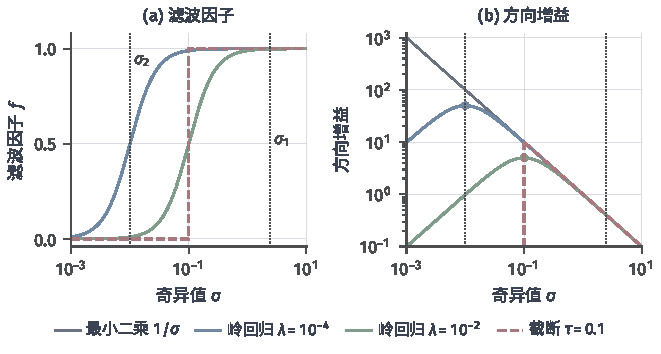
\includegraphics[width=112mm]{figures/01-basic-mathematics/03-vectors-matrices-and-multivariate-functions/matplotlib/c5-ridge-tsvd-filter-factors/figure.pdf}
 \caption{岭回归与截断SVD沿奇异方向的作用。(a)滤波因子：岭回归$f=\sigma^2/(\sigma^2+\lambda)$在$\sigma=\sqrt\lambda$处取$1/2$并连续过渡，截断SVD在阈值$\tau$处由$0$跳到$1$。(b)方向增益：最小二乘为$1/\sigma$，岭回归为$\sigma/(\sigma^2+\lambda)$，圆点是峰值$1/(2\sqrt\lambda)$；截断后小于$\tau$的方向增益为零。竖虚线是示例~\ref{ex:ls-tsvd-steps}中矩阵的两个奇异值。}
 \label{fig:ls-ridge-tsvd-filter-factors}
\end{figure}

\paragraph{算法实现}
这里要区分两件事。第~\ref{sec:ls-qr-method}节的正交算法改善的是同一问题的计算过程；正则化则主动修改了问题，以控制敏感性。计算路线有三条。第一条对堆叠矩阵$\bm F$作Householder QR再回代，适用于任意$\bm L$。第二条只用于$\bm L=\bm I$：先作一次SVD，算出$c_i=\bm u_i^\top\bm b$，此后每个$\lambda$只需按式~\eqref{eq:matrix-analysis-ridge-filter-factor}乘滤波因子，扫描多个参数时最省。第三条对$\bm A^\top\bm A+\lambda\bm L^\top\bm L$作Cholesky分解（第~\ref{sec:ls-cholesky}节），再依次前代、回代；大型问题还可以把LSQR（第~\ref{sec:ls-lsqr}节）用于增广问题~\eqref{eq:ls-augmented-system}。

\begin{example}[直线拟合的岭回归]
\label{ex:ls-ridge-line-fit}
沿用示例~\ref{ex:ls-line-least-squares}的$\bm A=\left[\begin{smallmatrix}1&0\\1&1\\1&2\end{smallmatrix}\right]$与$\bm b=(1,2,2)^\top$，取$\lambda=1$，走Cholesky路线。正则化后的方程为
\[
 \begin{bmatrix}4&3\\3&6\end{bmatrix}\bm x=\begin{bmatrix}5\\6\end{bmatrix},
\]
分解得$l_{1,1}=2$，$l_{2,1}=1.5$，$l_{2,2}=\sqrt{6-1.5^2}\approx1.9365$。前代得$y_1=2.5$，$y_2=(6-1.5\times2.5)/1.9365\approx1.1619$；回代得$x_2=1.1619/1.9365=0.6$，$x_1=(2.5-1.5\times0.6)/2=0.8$。于是$\bm x_\lambda=(0.8,0.6)^\top$，拟合值$(0.8,1.4,2.0)^\top$，残差$(0.2,0.6,0)^\top$。核验正则化的正规残差：$\bm A^\top\bm r=(0.8,0.6)^\top$恰等于$\lambda\bm x_\lambda$，两者之差为零。与最小二乘解$(7/6,1/2)^\top$相比，残差平方由$1/6$增至$0.4$，解的长度由$1.269$降为$1$。按SVD路线，$\sigma_1^2\approx7.162$、$\sigma_2^2\approx0.838$，滤波因子为$f_1\approx0.877$、$f_2\approx0.456$：$\sigma_2^2$与$\lambda$相当，第二个方向被压掉约一半。
\end{example}

\paragraph{算法分析}
Cholesky路线的条件数是$\kappa_2(\bm F)^2$。岭回归中$\kappa_2(\bm F)=\bigl((\sigma_1^2+\lambda)/(\sigma_d^2+\lambda)\bigr)^{1/2}\leq(1+\sigma_1^2/\lambda)^{1/2}$（$\sigma_d$为第$d$个奇异值，秩亏时为零），即使$\bm A$秩亏也有界，所以只在$\lambda$不太小、$(1+\sigma_1^2/\lambda)u\ll1$时这条路线与QR同样可靠。无论哪条路线，结果都要回到正则化目标核验，分别报告拟合误差$\lVert\bm A\bm x_\lambda-\bm b\rVert_2$与惩罚大小$\lVert\bm L\bm x_\lambda\rVert_2$，正规残差应检查$\bm A^\top(\bm b-\bm A\bm x_\lambda)-\lambda\bm L^\top\bm L\bm x_\lambda$，而不是原问题的$\bm A^\top\bm r$。

\subsection{截断SVD求解}
\label{sec:ls-tsvd-solve}

\paragraph{主要思想}
截断SVD只在保留的前$k$个奇异方向上取倒数，舍弃其余方向：
\[
 \bm x_k=\sum_{i=1}^k\frac{\bm u_i^\top\bm b}{\sigma_i}\,\bm v_i=\bm A_k^\dagger\bm b,\qquad 1\leq k\leq r,
\]
其中$\bm A_k=\sum_{i\leq k}\sigma_i\bm u_i\bm v_i^\top$是第~\ref{sec:ls-low-rank-approximation}节的截断SVD（式~\eqref{eq:matrix-analysis-truncated-svd}），$\bm A_k^\dagger\bm b$是以$\bm A_k$代替$\bm A$后的最小范数最小二乘解。它与最佳低秩逼近共用同一个分解，目的却不同：低秩逼近要重建矩阵，截断求解要从带误差的观测中稳定地恢复输入。

\paragraph{算法实现}
先求经济型SVD，并算出$c_i=\bm u_i^\top\bm b$。然后按阈值$\tau$取$k=\#\{i:\sigma_i>\tau\}$，令$\bm x_k=\sum_{i\leq k}(c_i/\sigma_i)\bm v_i$。最后由$\bm A\bm x_k=\sum_{i\leq k}c_i\bm u_i$读出拟合值，残差不必再乘$\bm A$就能得到；换一个阈值只需增减和式中的项。

\begin{example}[近共线设计的截断求解]
\label{ex:ls-tsvd-steps}
设计矩阵的两列为$(1,1,1)^\top$与$(1,1.01,0.99)^\top$，观测$\bm b=(1,1.1,0.9)^\top$。SVD给出$\sigma_1\approx2.449$、$\sigma_2\approx0.0100$，$\bm v_1\approx(1,1)^\top/\sqrt2$，$\bm v_2\approx(1,-1)^\top/\sqrt2$；投影系数$c_1\approx1.733$，$c_2\approx-0.134$。取$\tau=0.1$，只有$\sigma_1$超过阈值，$k=1$。于是$\bm x_1=(c_1/\sigma_1)\bm v_1\approx0.7073\,\bm v_1\approx(0.50,0.50)^\top$。$\bm b$在列空间内，残差全部来自舍弃的方向，$\lVert\bm b-\bm A\bm x_1\rVert_2=|c_2|\approx0.134$；正规残差$\bm A^\top(\bm b-\bm A\bm x_1)=\sigma_2c_2\bm v_2$的长度约为$0.0013$，不为零，$\bm x_1$不是原问题的最小二乘解。若不截断，第二个方向贡献$(c_2/\sigma_2)\bm v_2\approx-13.4\,\bm v_2$，得到精确拟合的$(-9,10)^\top$。
\end{example}

\paragraph{算法分析}
设观测由真实输入加噪声得到。截断解的误差与拟合损失都可以按奇异方向分开。

\begin{theorem}[截断SVD的误差分解]
\label{thm:ls-tsvd-error-decomposition}
设$\bm b=\bm A\bm x_{\mathrm{true}}+\bm e$，$\bm x_{\mathrm{true}}\in\operatorname{range}\bm A^\top$，$1\leq k\leq r$。则
\[
 \bm x_k-\bm x_{\mathrm{true}}=\sum_{i=1}^k\frac{\bm u_i^\top\bm e}{\sigma_i}\,\bm v_i-\sum_{i=k+1}^r(\bm v_i^\top\bm x_{\mathrm{true}})\,\bm v_i ,
\]
两项正交，第一项的长度不超过$\lVert\bm e\rVert_2/\sigma_k$。此外
\[
 \lVert\bm b-\bm A\bm x_k\rVert_2^2=\lVert\bm b-\bm A\hat{\bm x}\rVert_2^2+\sum_{i=k+1}^rc_i^2,\qquad
 \bm A^\top(\bm b-\bm A\bm x_k)=\sum_{i=k+1}^r\sigma_ic_i\bm v_i ,
\]
其中$\hat{\bm x}$为任一最小二乘解。
\end{theorem}
\begin{proof}
由$c_i=\sigma_i\bm v_i^\top\bm x_{\mathrm{true}}+\bm u_i^\top\bm e$，$\bm x_k=\sum_{i\leq k}(\bm v_i^\top\bm x_{\mathrm{true}}+\bm u_i^\top\bm e/\sigma_i)\bm v_i$；而$\bm x_{\mathrm{true}}=\sum_{i\leq r}(\bm v_i^\top\bm x_{\mathrm{true}})\bm v_i$，相减即得误差式。两项落在互相正交的$\bm v_i$上；第一项长度的平方为$\sum_{i\leq k}(\bm u_i^\top\bm e)^2/\sigma_i^2\leq\lVert\bm e\rVert_2^2/\sigma_k^2$。残差$\bm b-\bm A\bm x_k=(\bm I-\bm A\bm A^\dagger)\bm b+\sum_{i>k}c_i\bm u_i$，两部分正交，前者就是最小二乘残差；再用$\bm A^\top\bm u_i=\sigma_i\bm v_i$与$\bm A^\top(\bm I-\bm A\bm A^\dagger)=\bm0$得正规残差。
\end{proof}

第一项是保留方向的噪声放大，界由$\sigma_k$而不是$\sigma_r$决定；第二项是舍弃方向上真实输入的全部损失。拟合的代价是残差平方多出被舍弃的$c_i^2$；主要计算代价是一次SVD，为$O(md^2)$量级。

\paragraph{与岭回归的比较}
岭回归连续地压低小奇异值方向，截断则把滤波因子直接取成$1$（$i\leq k$）或$0$（$i>k$），两者在图~\ref{fig:ls-ridge-tsvd-filter-factors}中分别是光滑曲线与阶梯。下面的例子在同一组数据上比较两者。

\begin{example}[岭回归与截断SVD的比较]
\label{ex:ls-regularization-response}
沿用示例~\ref{ex:ls-tsvd-steps}的数据，再把$\bm b$改为$(1,1.11,0.89)^\top$，这个扰动几乎全部落在$\bm u_2$上。各方法的结果为
\[
 \begin{array}{lccc}
  \text{方法} & \bm x & \lVert\bm r\rVert_2 & \lVert\Delta\bm x\rVert_2/\lVert\Delta\bm b\rVert_2\\[2pt]
  \text{最小二乘} & (-9,\,10)^\top & 0 & 100\\
  \lambda=10^{-4} & (-4.25,\,5.25)^\top & 0.067 & 50\\
  \lambda=10^{-2} & (0.41,\,0.59)^\top & 0.133 & 0.99\\
  k=1 & (0.50,\,0.50)^\top & 0.134 & 0.002
 \end{array}
\]
响应比就是第二个方向的增益：最小二乘为$1/\sigma_2=100$，岭回归为$\sigma_2/(\sigma_2^2+\lambda)$，截断后为零，剩下的$0.002$来自扰动在$\bm u_1$上的微小分量。精确拟合的大系数全部来自第二个方向；系数越稳定，残差越大，$\lambda=10^{-2}$的岭回归与$k=1$的截断已经很接近。
\end{example}

奇异值在某处明显下降时，截断位置有自然的选择，截断把可信与不可信的方向分得最清楚；奇异值缓慢衰减、没有间隔时，连续衰减的岭回归更平稳。阈值应联系噪声规模、截断处的奇异值间隔和任务目标，取$\tau$为数据误差的估计，就是只在第~\ref{sec:ls-pseudoinverse-rank-change}节意义下可辨认的方向上反演；它不等同于按机器精度判定精确秩，只有数据仅含舍入误差时两者才一致。

\paragraph{与低秩逼近的边界}
截断求解与第~\ref{sec:ls-low-rank-approximation}节的结论有明确的边界。$\bm A_k$在谱范数与Frobenius范数下是最佳秩$k$重建（定理~\ref{thm:matrix-analysis-best-low-rank}），但由定理~\ref{thm:ls-tsvd-error-decomposition}的正规残差，除非被舍弃的$c_i$全为零，$\bm x_k$不是原问题的最小二乘解；矩阵逼近的最优性又不涉及$\bm x_{\mathrm{true}}$与$\bm e$，更不能由它断言$\bm x_k$最接近未知的真实输入。所以截断求解要同时说明保留了哪些方向、噪声水平多大、允许多大的拟合损失。保留的方向本身是否可靠，还要看截断处的间隔$\sigma_k-\sigma_{k+1}$：间隔很小时，扰动可能使前$k$个奇异方向明显偏转，第~\ref{sec:ls-subspace-sensitivity}节的奇异值与子空间扰动界可以用来判断。
